%; whizzy chapter
% -initex iniptex -latex platex -format platex -bibtex jbibtex -fmt fmt
% 以上 whizzytex を使用する場合の設定。

%     Kansai Debian Meeting resources
%     Copyright (C) 2007 Takaya Yamashita
%     Thank you for Tokyo Debian Meeting resources

%     This program is free software; you can redistribute it and/or modify
%     it under the terms of the GNU General Public License as published by
%     the Free Software Foundation; either version 2 of the License, or
%     (at your option) any later version.

%     This program is distributed in the hope that it will be useful,
%     but WITHOUT ANY WARRANTY; without even the implied warranty of
%     MERCHANTABILITY or FITNESS FOR A PARTICULAR PURPOSE.  See the
%     GNU General Public License for more details.

%     You should have received a copy of the GNU General Public License
%     along with this program; if not, write to the Free Software
%     Foundation, Inc., 51 Franklin St, Fifth Floor, Boston, MA  02110-1301 USA

%  preview (shell-command (concat "evince " (replace-regexp-in-string "tex$" "pdf"(buffer-file-name)) "&"))
% 画像ファイルを処理するためにはebbを利用してboundingboxを作成。
%(shell-command "cd image200708; ebb *.png")

%%ここからヘッダ開始。

\documentclass[mingoth,a4paper]{jsarticle}
\usepackage{kansaimonthlyreport}
\usepackage[dvips]{xy}

% 日付を定義する、毎月変わります。
\newcommand{\debmtgyear}{2010}
\newcommand{\debmtgdate}{24}
\newcommand{\debmtgmonth}{01}
\newcommand{\debmtgnumber}{31}

\begin{document}

\begin{titlepage}

% 毎月変更する部分、本文の末尾も修正することをわすれずに

 第\debmtgnumber{}回 関西 Debian 勉強会資料

\vspace{2cm}

\begin{center}
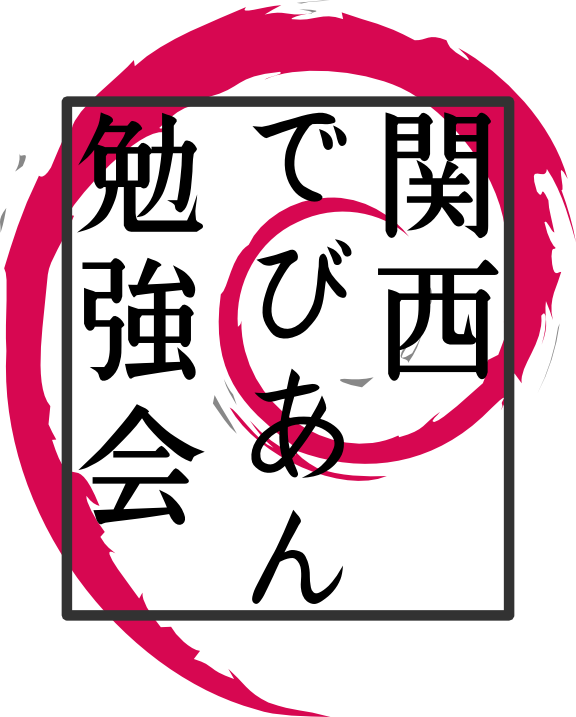
\includegraphics{image200802/kansaidebianlogo.png}
\end{center}

\begin{flushright}
\hfill{}関西 Debian 勉強会担当者 佐々木・倉敷・のがた \\
\hfill{}\debmtgyear{}年\debmtgmonth{}月\debmtgdate{}日
\end{flushright}

\thispagestyle{empty}
\end{titlepage}

\dancersection{Introduction}{Debian JP}

\subsection*{}%ロゴ用のスペース稼ぎ
 
関西 Debian 勉強会はDebian GNU/Linux のさまざまなトピック(新しいパッケー
ジ、Debian 特有の機能の仕組、Debian 界隈で起こった出来事、などなど)に
ついて話し合う会です。

目的として次の三つを考えています。
\begin{itemize}
      \item MLや掲示板ではなく、直接顔を合わせる事での情報交換の促進
      \item 定期的に集まれる場所
      \item 資料の作成
\end{itemize}

それでは、楽しい一時をお楽しみ下さい。

\clearpage

\begin{minipage}[b]{0.2\hsize}
 {\rotatebox{90}{\fontsize{80}{80}
{\gt 関西デビアン勉強会}}}
\end{minipage}
\begin{minipage}[b]{0.8\hsize}
\hrule
\vspace{2mm}
\hrule
\setcounter{tocdepth}{1}
\tableofcontents
\vspace{2mm}
\hrule
\end{minipage}

\dancersection{最近のDebian関係のイベント報告}{Debian JP}

\subsection{前回の関西 Debian 勉強会}

前回の関西 Debian 勉強会は 2009 年 12 月 27 日に大阪福島区民センターに
て開催されました。

発表は、
まささんによる、
GPS レシーバと EeePC を組み合わせて
自分の現在地をリアルタイムに表示させる「ハンドメイド GPS ロガーの構築」と、
%
たなかとしひささんによる、
Open Street Map の紹介と Debian での実演
「Debianを使って愉しむ Open Street Map 入門」でした。

関西 Debian 勉強会では、最近 GPS ロガーを持っている人が増えているわけですが、
今後ますます増えそうな気がします\footnote{%
というか、ついに佐々木も購入してしまいました(笑)}。%

\subsection{第 60 回東京エリア Debian勉強会 - BSP 2010/Tokyo}

1 月 23 日(昨日), 
第 60 回東京エリア Debian勉強会 - BSP 2010/Tokyo が開催されました。
この原稿を執筆している時点では未来の出来事なわけですが、
(恐らく)盛大に Bug Squash が行なわれた事と想像されます。

Debian の次期安定版、コードネーム Squeeze のリリースフリーズは
2010年 3 月が予定されています。
バグ潰しだけではなくドキュメント/po の翻訳などやっておきたい事がある人は
早めにやっつけてしまいましょう。

現在の RC バグの状況は
\url{http://bugs.debian.org/release-critical/} で確認できます。

\clearpage
\dancersection{Xenで作る自宅サーバ}{川江 浩}

\subsection{はじめに}
近年、CPUの性能がパワフルになるにつれて、高価なハードウェアを前提とした
仮想化技術がパーソナルベースでも使えるようになってきました。

そこで、脚光を浴びてきた仮想化技術の代表格であるXenを使って、インタネッ
ト関連のサーバ群を構築しましたので、DebianベースでXenの仮想サーバを構築
する時に注意することや、上記サーバ群を構築する際に思ったことをレポート
します。

また、以下の仕様はパーソナルベースでの運用を前提に構築したものです。仕
様を試そうとするときは、必ずデータ等のバックアップをとって自己責任で行っ
てください。より詳しく知りたい方は専門書を参照してください。

\subsection{Xenとは}
Xenは、仮想マシンソフトウェアの一つで、OSより1つの下の階層でハイパーバ
イザというプログラムを動かすものです。このタイプはハイパーバイザ型と呼
ばれ、「VMware Infrastrucure」などがあります。

他方、仮想マシンソフトウェアにはアプリケーションタイプと呼ばれるものが
あり、「VMware Workstation」「VirtualBox」「QEMU」が有名です。

\subsection{Xenの特徴}
Xenは仮想化するためのモデルとして、準仮想化と完全仮想化の2つを提供しています。
\begin{itemize}
\item 準仮想化(ParaVirtualization)\\
Xenでの準仮想化はハードウェアをエミュレートする代わりに、仮想マシン用のハードウェアを使用します。このハードウェアは操作をするためにハイパーバイザコールを呼び出します。ハイパーバイザコールは仮想マシン環境に対応し、OSはXen仮想ハードウェア用に修正する必要があります。

\item 完全仮想化(FullVirtualization)\\
Xenは完全仮想化機能も提供しています。この機能を利用すると、デフォルトのOSをそのままXen上で動作させることができます。
\end{itemize}

\subsection{Xenの形態}
XenはLinuxをベースに作られていますので、Xen用にコンパイルされたカーネルを利用します。このカーネルは起動時にハイパーバイザをロードし、その上にカーネルをロードします。イメージ的にはハイパーバイザ上を管理OSのDomainOが動き、そのOSに管理される形でゲストOSと呼ばれるDomainUが動きます。

\begin{itemize}
\item Domain-O (管理OS)以下DomO \\
      Xenを起動したOS。ハードウェアを管理し、ハイパーバイザ上で動作するゲストOSの管理を行う。
\item Domain-U (DomU-準仮想化)以下DomU \\
      Domain-Oによって起動、管理されるゲストOS。特に、準仮想化で動作する。
\item HVM Domain (HVM-完全仮想化)以下HVM \\
      Domain-Oによって起動、管理されるゲストOSであるが、完全仮想化であるHVM(Hardware Virtual Machine)で動作する。
\end{itemize}

%図形の挿入
\begin{figure*}[h!]
 \centering
 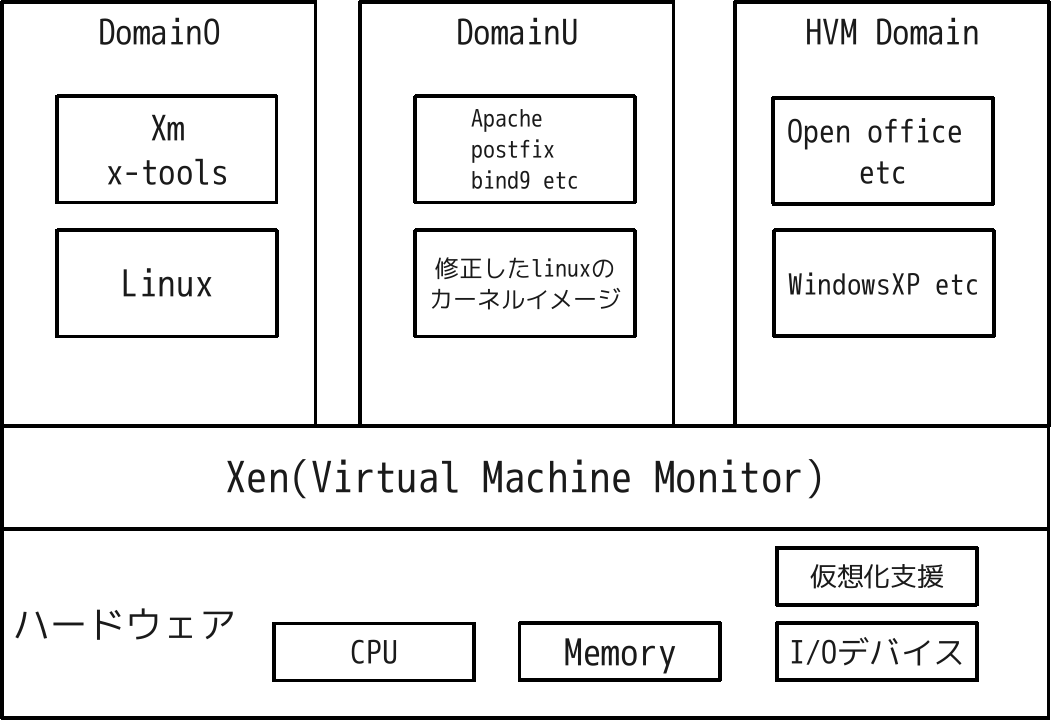
\includegraphics[scale=0.6]{image201001/xen-image.png}
 \caption{Xen のハイパーバイザモデルのイメージ}
\end{figure*}
\clearpage

\subsection{Xen の導入}
次に, Xen をインストールします. インストールは各アーキテクチャによって異なります. \footnote{詳しくは, 仮想化技術 Xen -概念と内部構造などを参照してください. 完全仮想化を目的にするのであれば Intel-VT や AMV-V が, CPU で仮想化支援機能を持っています. } ここでは, インテルをベースに Lenny の Xen カーネルイメージ 2.6.26 を以下の様にインストールします.

\begin{commandline}
# aptitude install xen-linux-system-2.6.26-2-xen-686 
\end{commandline}
また, Debian には DomU を作るツールも用意してありますので, これもインストールします.
\begin{commandline}
# aptitude install xen-tools
\end{commandline}
各インストールが済んだら, /xen/xen/xend-config.sxp ファイルの以下の箇所を変えます.
\begin{commandline}
(network-script 'network-bridge netdev=eth1')
(network-script 'network-bridge netdev=eth0')
\end{commandline}
再起動し, DomO の起動を確認します.
\begin{commandline}
# xm list
Name                 ID   Mem  VCPUs   State   Time (s)
Domain-0             0   1478     1   r-----    217.6
\end{commandline}

\subsection{DomU の設定}
Xen のツールを使ってゲスト OS を以下の手順で入れます. (etch や Ubuntu, CentOS も可能).
\begin{enumerate}
\item 設定ファイルの編集
\item xen-create-image の実行
\item DomU の起動
\end{enumerate}

\subsubsection{設定ファイルの編集}
設定ファイルは, /etc/xen-tools/xen-tools.conf です. 以下, DomU に Lenny をインストールものとして編集します.

%改ページ, 注意
\begin{commandline}
##
#  /etc/xen-tools/xen-tools.conf
##             (中略)
#  Output directory for storing loopback images.
#
#  If you choose to use loopback images, which are simple to manage but
# slower than LVM partitions, then specify a directory here and uncomment
# the line.
#
#  New instances will be stored in subdirectories named after their
# hostnames.
# 
##
dir = /home/xen (イメージファイルの保管場所です)
#              (中略)

##
#  Disk and Sizing options.
##
size   = 4Gb      # Disk image size.
#memory = 128Mb    # Memory size
memory = 384Mb    # Memory size
#swap   = 128Mb    # Swap size
swap   = 512Mb    # Swap size
# noswap = 1      # Don't use swap at all for the new system.
fs     = ext3     # use the EXT3 filesystem for the disk image.
#dist   = etch     # Default distribution to install.
dist   = lenny     # Default distribution to install.

#  Currently supported and tested distributions include:
#
# via Debootstrap:
#
#  Debian:
#   sid, sarge, etch, lenny.(他のディストリビューションの選択も可能)
#
#  Ubuntu:
#   edgy, feisty, dapper.
#
# via Rinse:
#   centos-4, centos-5.
#   fedora-core-4, fedora-core-5, fedora-core-6, fedora-core-7

##
# Networking setup values.
##
#
## Uncomment and adjust these network settings if you wish to give your
# new instances static IP addresses.
#
# gateway   = 192.168.1.1
gateway   = 192.168.0.1
# netmask   = 255.255.255.0
netmask   = 255.255.255.0
# broadcast = 192.168.1.255
broadcast = 192.168.0.255
#(ネットワークはご自由に)

#(以下はデフォルトにしました)
# Default kernel and ramdisk to use for the virtual servers
#
kernel      = /boot/vmlinuz-`uname -r`
initrd      = /boot/initrd.img-`uname -r`

#  The architecture to use when using debootstrap, rinse, or rpmstrap.
#
#  This is most useful on 64 bit host machines, for other systems it
# doesn't need to be used.
#
# arch=[i386|amd64]
#

# The default mirror for debootstrap to install Debian-derived distributions
#
mirror = http://ftp.jp.debian.org/debian/

#  If you're using the lenny or later version of the Xen guest kernel you will
# need to make sure that you use 'hvc0' for the guest serial device,
# and 'xvdX' instead of 'sdX' for serial devices.
#
#  You may specify the things to use here:
#
serial_device = hvc0 #default
# serial_device = tty1
#
disk_device = xvda #default
# disk_device = sda

#  Here we specify the output directory which the Xen configuration
# files will be written to, and the suffix to give them.
#
#  Historically xen-tools have created configuration files in /etc/xen,
# and given each file the name $hostname.cfg.  If you want to change
# that behaviour you may do so here.
#
# output    = /etc/xen
# extension = .cfg
#
\end{commandline}

\subsubsection{xen-create-image の実行}
次に, DomU のイメージを作ります. 同時に DomU に割り当てる IP アドレスをオプションで指定します. 例えば, アドレスを 192.168.0.2, ホストネームを dns とするなら以下のようにします.
\begin{commandline}
# xen-create-image --ip 192.168.0.2 --hostname dns
\end{commandline}
DomU の制作には, イメージディスクの大きさやネットワークの状況によって異なりますが, 自分の環境では 10G のイメージで 30 分ぐらいでした.

\subsubsection{DomU の起動}
無事に, インストールができたら起動して, 稼働状況を見てみましょう.
\footnote{Xen には管理用ツールとして「 xm 」などがあります. 詳しくは, Xen 徹底入門などを参照してください. }
\begin{commandline}
# xen create -c dns.cfg
# xm list
 Name                                        ID   Mem VCPUs      State   Time (s)
 Domain-0                                     0  1478     4     r-----    429.8
 dns                                          5   384     1     -b----     10.5
 mail                                         2   384     1     -b----    123.6
 www                                          4  1792     1     -b----     23.1
\end{commandline}
起動してくる画面は, 全くの初期状態でログインプロンプトしか出ません. root でログインしてパスワードとユーザを作成します.
\begin{commandline}
# passwd
# adduser ipv6waterstar
\end{commandline}
\subsubsection{バックアップ, 他}
また, DomU をデフォルトでインストールした場合, DomO の/home/xen/domain に各 DomU のドメインごとにメージファイルが置かれます. また, 設定ファイルは/etc/xen に  ".cfg"ファイルとして保存されます.

従って, 例えば何らかの設定ミスをして DomU が起動不能になっても, 上記のイメージと設定ファイルのバックアップがあれば, 各ディレクトリと設定ファイルをそのままコピーし直すだけで, 同じ環境の DomU を復元できます.

また, 管理用の DomO はセキュリティの関係からプロセス数が少ない方がいいのですが, 後述のように設定ファイルを多数, 作成する場合のことも考えると, GUI で操作ができるなどの利点から, gnome などをインストールすることを勧めます.


\subsection{Xen のネットワークの概要}
Xen は仮想インターフェイスをベースにしたネットワーク機能を持っています.

具体的には, DomU の各ホストを直接外部ネットワークに接続するブリッジ経由の接続. 仮想インターフェイスを通して, DomO のルーティングし, ネットワークインターフェイスに出力するブリッジを経由しない接続 (NAT 接続) の二つの形態があります.

ブリッジ経由の接続のイメージはハードウェア上に, DomO と複数の DomU の仮想 PC があって, それぞれが対等にネットワークハブで繋がっているような状態です.

今回は, 各 DomU サーバをインターネットサーバとして運用したいので, 仮想インターフェイスを使って直接, セグメントが異なる外部ネットワークに接続できるブリッジ経由の接続でネットワークを構成します.

DomU は仮想マシンを作成するときに, IP アドレスを割り当てたので特別な設定は必要ありません. 同時に, Mac アドレスも各仮想インターフェイスごとに自動的に割り当てられます.

また, IP アドレスを後から変更したいときなどは/etx/xen 以下の".cfg"ファイルを書き換えます.

例  dns.cfg
%改ページ  注意
\begin{commandline}
#
# Configuration file for the Xen instance www, created
# by xen-tools 3.9 on Tue Nov 17 10:35:03 2009.
#

#
#  Kernel + memory size
#
kernel      = '/boot/vmlinuz-2.6.26-2-xen-686'
ramdisk     = '/boot/initrd.img-2.6.26-2-xen-686'
memory      = '384'(メモリーの容量の変更も可能)

#
#  Disk device (s).
#
root        = '/dev/xvda2 ro'
disk        = [
                  'file:/home/xen/domains/www/swap.img,xvda1,w',
                  'file:/home/xen/domains/www/disk.img,xvda2,w',
              ]


#
#  Hostname
#
name        = 'dns'(ホスト名)

#
#  Networking
#
vif         = [ 'ip=192.168.0.2,mac=00:12:34:56:78:9A' ]
(アドレスの変更も可能ですが, DomU の interfaces を書き換えているときはそちらも書き換えてください)

#
#  Behaviour
#
on_poweroff = 'destroy'
on_reboot   = 'restart'
on_crash    = 'restart'
\end{commandline}

\subsubsection{各インターネットサーバの設定する前の注意事項}
次に, DNS, Mail サーバ, Web サーバのパッケージを, 各 DomU にインストールします.

インストールは, 仮想マシンでもノーマルのインストールと変わりません. ただ, Xen のネットワーク構成は独特の「癖」のようなものがあります. 以下, いくつか例を挙げます.
\begin{enumerate}
\item NTP を使った時間の設定 
\item SSH でのログイン
\item その他 
\end{enumerate}

\subsubsection{NTP を使った時間の設定}
DomU は Dom0 からのみ時刻を更新できるという Xen の仕様なので, Dom0 で時刻を合わせていれば, DomU も正確な時刻を得ることができます. ただ, DomU で ntpd や ntpdate を実行するのであれば, 時刻同期できないことがあります.

普通に DomU で時計を合わせるのであれば, Aisa/Tokyo に合わせることで日本時間にできます (デフォルトでは UTC).
\begin{commandline}
# dpkg-reconfigure tzdata
# date
  Tue Jan 24 15:00:00 JST 2010
\end{commandline}

また, DomU で NTP 等を使うのであれば, DomU の/etc/sysctl.conf に{\tt xen.independent\_wallclock=1}を加えて再起動してください.

\subsubsection{SSH でのログイン}
Xen で SSH を使って, ネットワーク越しにログインする場合も通常と同じでが, インストールしたばかりの DomU は何も入っていないので, そのままではエラーになります.

具体的には, まず DomU に SSH をインストールします (ポート番号の変更などはお好みで).
\begin{commandline}
# aptitude install ssh
\end{commandline}

次にローカルから SSH を使ってログインしようとしても, 以下のエラーがでます.
\begin{commandline}
$ ssh mail.kinsen.gr.jp
  ipv6waterstar@dns.kinsen.gr.jp's password: 
  PTY allocation request failed on channel 0
\end{commandline}

原因は, xen-tools を使った DomU の構築で「 udev をインストールしないため」に起こります. 従って, DomU に udev をインストールすることで解決します.
\begin{commandline}
# aptitude install udev
\end{commandline}

\subsubsection{その他}
その他, Xen でサーバを運用するときにいくつか気づいたものを挙げます.

まず, DomO と DomU がブリッジ経由で接続している場合, iptables で FORWARD を使うと DomU からネットワークに繋がらない現象が起こります (理由は不明).

また, 完全仮想化でゲスト OS を動かそうとするのであれば, CD をゲスト OS からマウントし, VNC などを立ち上げてインストールする必要があります (検証はしてませんので, 可能かどうかは不明).

詳しくは, 以下のドキュメント等を参照してください.
\begin{itemize}
\item \url{http://wiki.debian.org/Xen}
\end{itemize}

\subsection{各インターネットサーバの設定}
次に, 各インターネットサーバの設定の手順を説明します. ここでの環境は, グローバル IP アドレスが 1 つで, インターネットには電話会社から提供されているルータで外部ネットワークに, 繋がっていることを前提とします.

\subsubsection{DNS の概要}
DNS サーバはホスト名と IP アドレスを対応させたゾーンと呼ばれるファイルを持ち, ホスト名の検索に対して対応する IP アドレスを返します. また, ゾーンファイルの内容を他のサーバに転送します.

具体的に www.kinsen.gr.jp というホスト名に対応する IP アドレスを (再帰) 検索する場合, まず, jp ドメインの IP アドレスを問い合わせる必要があります. そのために, ルートサーバで jp ドメインの IP アドレスを検索し, jp サーバに接続します. 同様に, jp に属する gr ドメインの IP アドレスを検索し, さらには gr ドメインに属する kinsen そして www と順次, 各 IP アドレスを検索し, 各サーバに接続していきます. そして最終的に, www.kinsen.gr.jp の IP アドレスが 203.141.158.41 である事がわかります.

Debian には DNS サーバとして bind9 のパッケージが用意されています. 以下, インストールと設定を行います.

\subsubsection{DNS の設定}
bind9, bind9utils パッケージをインストールします.
\begin{commandline}
# aptitude install bind9
# aptitude install bind9utils
\end{commandline}
今回はパーソナルユースなので 1 個のグローバル IP アドレスを使うことを前提とし, ネームサーバの設定には view や match-client を使います (例として, 内部ゾーンで, 192.168.0.0/24 ネットワーク内に各サーバを, グローバルアドレスとして 203.141.158.41 を使うものとします).

view は指定の IP アドレスやネットワークごとに, 個別のオプションとゾーンデータを提供します.

具体的には, acl で IP アドレスとネットワークを指定し, match-clients で acl にマッチするクライアントと, その他のクライアントごとに別々ゾーンを提供します. これを利用し, 1 台のサーバで内部用 (acl にマッチする) と外部用 (acl にマッチしない) の DNS を構築します.

なお, グローバル IP アドレスが複数の場合は, 各 DomU にグローバル IP アドレスを設定してください. \footnote{詳しくは, DNS BIND 第 5 版などを参照してください. }

\subsubsection{view の設定}
通常, BIND で view を設定する場合, named.conf に view や acl, match-clients の設定を書き加えます. だだ, Debian では, named.conf.options や named.conf.local などのファイルがありますので, それらを利用します.

まず, named.conf に以下のように書き換え, include を使って設定ファイルを挿入するようにします.
\begin{commandline}
// This is the primary configuration file for the BIND DNS server named.
//
// Please read /usr/share/doc/bind9/README.Debian.gz for information on the 
// structure of BIND configuration files in Debian, *BEFORE* you customize 
// this configuration file.
//
// If you are just adding zones, please do that in /etc/bind/named.conf.local
include "/etc/bind/named.conf.acl";  //view を使うアドレスの範囲を設定する
include "/etc/bind/named.conf.options";  //BIND の調整ためのオプション
view "internal"{  // 内部用ゾーンの設定
	match-clients { localnet; };  // 内部ゾーンの適用範囲の設定
	recursion yes;
include "/etc/bind/named.conf.conf";  // 内部用ゾーンの初期設定
include "/etc/bind/named.conf.local";  // 内部用ゾーンのローカル設定
};
view "external" {  // 外部用ゾーンの設定
	match-clients { any; };  // 外部ゾーンの適用範囲の設定
	recursion no;
include "/etc/bind/named.conf.view"; // 外部用ゾーンのローカル設定
};
\end{commandline}

\subsubsection{named.conf.acl の設定}
acl ステートメントでは, アドレスマッチリストを設定します.

named.conf.acl の内容は以下の通り
\begin{commandline}
acl localnet{ 
	192.168.0.0/24; 
	127.0.0.1; 
};
\end{commandline}

\subsubsection{named.conf.options の設定}
options ステートメントでは, BIND の動作に関わるもろもろのオプションを設定します.

named.conf.options の内容は以下の通り
\begin{commandline}
options {
	directory "/var/cache/bind";

	// If there is a firewall between you and nameservers you want
	// to talk to, you may need to fix the firewall to allow multiple
	// ports to talk.  See http://www.kb.cert.org/vuls/id/800113

	// If your ISP provided one or more IP addresses for stable 
	// nameservers, you probably want to use them as forwarders.  
	// Uncomment the following block, and insert the addresses replacing 
	// the all-0's placeholder.

	forwarders {
		123.456.789.001; 123.456.789.002;
            //ISP で指定された DNS に代理問い合わせを要求するアドレスを記入します.
	 };

	allow-query { any; };  // 問い合わせ可能なホストを無制限に
	allow-transfer { localnet; };  // 転送先を限定
	version "no version";  // バージョン表示を無効に
	auth-nxdomain no;    # conform to RFC1035
	listen-on-v6 { any; };

};
\end{commandline}

\subsubsection{named.conf.conf の設定}
このファイルはもとの named.conf (初期設定) ファイルです.

named.conf.conf の内容は以下の通り.
\begin{commandline}
// prime the server with knowledge of the root servers
zone "." {
	type hint;
	file "/etc/bind/db.root";
};

// be authoritative for the localhost forward and reverse zones, and for
// broadcast zones as per RFC 1912

zone "localhost" {
	type master;
	file "/etc/bind/db.local";
};

zone "127.in-addr.arpa" {
	type master;
	file "/etc/bind/db.127";
};

zone "0.in-addr.arpa" {
	type master;
	file "/etc/bind/db.0";
};

zone "255.in-addr.arpa" {
	type master;
	file "/etc/bind/db.255";
};
\end{commandline}

\subsubsection{named.conf.local の設定}
ローカルネット用の初期設定ファイル.

named.conf.local の内容は以下の通り
\begin{commandline}
//
// Do any local configuration here
//
zone "kinsen.gr.jp" {
	type master;
	file "/etc/bind/db.in-kinsen.gr.jp"; // 内部順引きゾーンテーブル
};
zone "0.168.192.in-addr.arpa" {
	type master;
	file "/etc/bind/db.192.168.0"; // 内部逆引きゾーンテーブル
};
// Consider adding the 1918 zones here, if they are not used in your
// organization
//include "/etc/bind/zones.rfc1918";
\end{commandline}

以下は各ゾーンファイルの設定例です.
\begin{enumerate}
\item 順引きゾーンテーブル
\begin{commandline}
;
; BIND data file for kinsen.gr.jp
;
$TTL	86400
@	IN	SOA	dns.kinsen.gr.jp. root.dns.kinsen.gr.jp. (
		              1		; Serial
			   1800		; Refresh
			    900		; Retry
			 604800		; Expire
			   1200 )	; Negative Cache TTL

                IN      NS      dns

; localhost
localhost       IN      A       127.0.0.1
localhost       IN      AAAA   ::1

; Mail exchange
                IN      MX   0  mail.kinsen.gr.jp.
;
; Host entry
;
noren           IN      A       192.168.0.1
;               IN      AAAA    2001:
dns             IN      A       192.168.0.2
;               IN      AAAA    2001:
mail            IN      A       192.168.0.3
;               IN      AAAA    2001:
www             IN      A       192.168.0.4
;               IN      AAAA    2001:
;
; Alias
;
;www            IN      CNAME   noren
;
; Domain
@               IN      A       192.168.0.2
                IN      MX 0    mail
\end{commandline}
\item 逆引きゾーンテーブル
\begin{commandline}      
;
;BIND data file for 219.117.222 network
;
$TTL    86400
@       IN      SOA     dns.kinsen.gr.jp. root.dns.kinsen.gr.jp. (
                              1         ; Serial
                           1800         ; Refresh
                            900         ; Retry
                         604800         ; Expire
                           1200 )       ; Negative Cache TTL

                IN      NS      dns
;
; Host entry
;
1		IN      PTR     noren.kinsen.gr.jp.
2		IN      PTR     dns.kinsen.gr.jp.
3		IN      PTR     mail.kinsen.gr.jp.
4		IN      PTR     www.kinsen.gr.jp.
\end{commandline}
\end{enumerate}

\subsubsection{named.conf.view の設定}
グローバルネット用の初期設定ファイルです.
named.conf.view の設定は以下の通り
\begin{commandline}   
zone "." {
	type hint;
	file "/etc/bind/db.root";
};
zone "kinsen.gr.jp"{
	type master;
	file "/etc/bind/db.out-kinsen.gr.jp"; // 外部順引きゾーンテーブル
	allow-transfer{ 
		localnet; 
		123.456.789.001; 
		123.456.789.002; 
	};
};
zone "158.141.203.in-addr.arpa"{
	type master;
	file "/etc/bind/db.203.141.158"; // 外部逆引きゾーンテーブル
	allow-transfer{ 
		localnet;
		123.456.789.001;
		123.456.789.002; 
	};
};
\end{commandline}
以下は各ゾーンテーブルの設定例です.
\begin{enumerate}
\item 順引きゾーンテーブル
\begin{commandline}
;
; BIND data file for kinsen.gr.jp
;
$TTL	86400
@	IN	SOA	dns.kinsen.gr.jp. root.dns.kinsen.gr.jp. (
		              1		; Serial
			   1800		; Refresh
			    900		; Retry
			 604800		; Expire
			   1200 )	; Negative Cache TTL

		IN	NS	dns

; localhost
localhost       IN      A       127.0.0.1
localhost       IN      AAAA    ::1

; Mail exchange
        	IN      MX   0 mail.kinsen.gr.jp.
;
; Host entry
;
noren           IN      A      203.141.158.41
;               IN      AAAA   2001:
dns             IN      A      203.141.158.41
;               IN      AAAA   2001:
mail            IN      A      203.141.158.41
;               IN      AAAA   2001:
www             IN      A      203.141.158.41
;               IN      AAAA   2001:
;
; Domain
@               IN      A       203.141.158.41
                IN      MX 0    mail
\end{commandline}
\item 逆引きゾーンテーブル
\begin{commandline}
;
;BIND data file for 203.141.158 network
;
$TTL    86400
@       IN      SOA     dns.kinsen.gr.jp. root.dns.kinsen.gr.jp. (
                              1         ; Serial
                           1800         ; Refresh
                            900         ; Retry
                         604800         ; Expire
                           1200 )       ; Negative Cache TTL

                IN      NS      dns
;
; Host entry
;
41		IN      PTR     noren.kinsen.gr.jp.
41		IN      PTR     dns.kinsen.gr.jp.
41		IN      PTR     mail.kinsen.gr.jp.
41		IN      PTR     www.kinsen.gr.jp.
\end{commandline}
\end{enumerate}
以上の設定が終わったら, BIND を再読み込み, 再起動します.
\begin{commandline}
# /etc/init.d/bind9 reload      注ー必ず再読み込みからしてください.
# /etc/init.d/bind9 restart  再読み込みでエラーがでたら必ず修正してください.
\end{commandline}
\clearpage

正常に読み込みが終わったら設定内容を dig や nslookup を使って確かめます.
\begin{commandline}
$ dig @localhost dns.kinsen.gr.jp (ホスト名はいろいろ試してください)
; <<>> DiG 9.5.1-P3 <<>> @localhost dns.kinsen.gr.jp
; (2 servers found)
;; global options:  printcmd
;; Got answer:
;; ->>HEADER<<- opcode: QUERY, status: NOERROR, id: 55957
;; flags: qr aa rd ra; QUERY: 1, ANSWER: 1, AUTHORITY: 1, ADDITIONAL: 0

;; QUESTION SECTION:
;dns.kinsen.gr.jp.              IN      A

;; ANSWER SECTION:
dns.kinsen.gr.jp.     86400     IN      A       192.168.0.2

;; AUTHORITY SECTION:
kinsen.gr.jp.         86400     IN      NS      dns.kinsen.gr.jp.

;; Query time: 0 msec
;; SERVER: 127.0.0.1#53 (127.0.0.1)
;; WHEN: Thu Jan 21 07:26:57 2010
;; MSG SIZE  rcvd: 64

$ dig @localhost kinsen.gr.jp MX (メールについても確認します)
; <<>> DiG 9.5.1-P3 <<>> @localhost kinsen.gr.jp MX
; (2 servers found)
;; global options:  printcmd
;; Got answer:
;; ->>HEADER<<- opcode: QUERY, status: NOERROR, id: 640
;; flags: qr aa rd ra; QUERY: 1, ANSWER: 1, AUTHORITY: 1, ADDITIONAL: 2

;; QUESTION SECTION:
;kinsen.gr.jp.                  IN      MX

;; ANSWER SECTION:
kinsen.gr.jp.           86400   IN      MX      0 mail.kinsen.gr.jp.

;; AUTHORITY SECTION:
kinsen.gr.jp.           86400   IN      NS      dns.kinsen.gr.jp.

;; ADDITIONAL SECTION:
mail.kinsen.gr.jp.      86400   IN      A       192.168.0.3
dns.kinsen.gr.jp.       86400   IN      A       192.168.0.2

;; Query time: 0 msec
;; SERVER: 127.0.0.1#53 (127.0.0.1)
;; WHEN: Thu Jan 21 07:25:15 2010
;; MSG SIZE  rcvd: 101

$ nslookup -type=mx kinsen.gr.jp (このコマンドでもいいです)
Server:         192.168.0.2
Address:	192.168.0.2#53

kinsen.gr.jp	mail exchanger = 0 mail.kinsen.gr.jp.
\end{commandline}



\subsection{Mail サーバの設定}
Mail サーバはメールの送受信を行います. 具体的には 2 つの機能に分別できます.
\begin{itemize}
\item MTA (Mail Transfer Agent  メール転送エージェント)\\
ユーザが送信したメールを受け取って, 他のサーバとバケツリレー式に目的地まで配送したり, 届いたメールを保管する機能
\item MDA (Mail Delivery Agent  メール配送エージェント)\\
振り分けられたメールをサーバ内のユーザや別のサーバへ配送する機能      
\end{itemize}

Debian では Exim がデフォルトのメールサーバになっていますが, インストールしたばかりの DomU にはインストールされていません. そこで, 今回は設定が容易で, 柔軟性も高く, ドキュメントも豊富な MTA の postfix をインストールします. \footnote{より詳しくは, Postfix 詳解  MTA の理解とメールサーバの構築, 運用を参照してください. }

また, Mail サーバからメールを取り出すために MDA は postfix と相性のよい Dovecot にし, IMAP プロトコルを使用します.

\subsubsection{postfix の設定}
次に, postfix をインストールし, 大まかな設定を dpkg-reconfitgure postfix で行い, 詳細な設定は後述の/etc/postfix/ の main.cf で直接, 書き換えるようにします.

\begin{commandline}
# aptitude install postfix
# dpkg-reconfitgure postfix 
\end{commandline}

以下, コンソールに設定画面が表示されます. 最初にサイトのタイプ, 次に各完全修飾ドメイン名, ルートやポストマスターとしてメールを受け取るユーザ, メールを受け取ることのできるその他のドメイン, メールの同期, 送信可能なネットワークの範囲, メールボックスのサイズ, 使用するプロトコルの種類などを環境に合わせて設定します.
\begin{commandline}
1.General type of mail configuration: Internet Site

2.System mail name: mail.kinsen.ge.jp

3.Root and postmaster mail recipient: ipv6waterstar

4.Other destinations for mail: mail.kinsen.gr.jp, kinsen.gr.jp, localhost

5.Force synchronous updates on mail queue?: No

6.Local networks: 127.0.0.0/8

7.Mialbox size limit (bytes): 0

8.Local address extension character: +

9.Internet protocols to use: all
\end{commandline}

\subsubsection{Maildir の設定}
また, 受信したメールを Mail ディレクトリで扱うように設定します. Maildir は保管する受信メールの取扱いが容易で, dovecot でも同様に扱うことができます.
\begin{commandline}
# postconf -e "home_mailbox = Maildir/"
# postconf -e "mailbox_command ="
\end{commandline}

\subsubsection{再起動とテスト}
大まかな設定が終わったら, 設定を読み込んでテストをしてみましょう.
\begin{commandline}
# /etc/init.d/postfix reload
# /etc/init.d/postfix restart
\end{commandline}
テストは telnet を使います. ただし, DomU には Telnet はインストールされていませんので, インストールしておいてください.
\begin{commandline}
# telnet localhost 25
  Trying 127.0.0.1...
  Connected to localhost.
  Escape character is '^]'.
  220 mail.kinsen.gr.jp ESMTP Postfix (Debian/GNU)
\end{commandline}
以上のようにでれば正常です. 引き続き自分宛にメールを送ってみましょう.
\begin{commandline}
  mail from: ipv6waterstar@kinsen.gr.jp
  rcpt to: ipv6waterstar@gmail.com
  data
  To: ipv6waterstar@gmail.com
  From: ipv6waterstar@kinsen.gr.jp
  Subject: Test
  This is my frist email on debian. Is it successed to send your mail?
       (本文ができたら)
  .    (を入力し)
  quit (で終了しましょう)
\end{commandline}

\subsubsection{main.cf の設定}
次に, メールサーバを立ち上げた場合, 気になるのは spam などの迷惑メール対策です. postfix は main.cf で詳細な設定が可能で, spam についてもアンチ spam 用の設定があります.

以下, main.cf の該当箇所を書き換えます.
\begin{commandline}
smtpd_recipient_restrictions = reject_invalid_hostname,
        reject_unknown_recipient_domain,
        reject_unauth_destination,
        reject_rbl_client sbl.spamhaus.org,
        permit

smtpd_helo_restrictions = reject_invalid_helo_hostname,
        reject_non_fqdn_helo_hostname,
        reject_unknown_helo_hostname (この設定を入れると, proxy 経由のメールが受け取れなくなります)
\end{commandline}
また, RBL (spam のブラックリスト) を使うこともできます.
\begin{commandline}
smtpd_client_restrictions = reject_rbl_client dnsbl.sorbs.net
\end{commandline}

\subsubsection{その他オプション (SMPT-AUTH, Sasl, TLS, サブミッション) の設定}
また, Postfix はオプションで様々なセキュリティの設定が行えますので, 代表的なものをいくつか設定します.
\begin{itemize}
\item SMPT-AUTH (メール送信に使うプロトコルである SMTP にユーザ認証機能を追加した仕様)\\
      SMTP がもともと認証を持たない仕様であったため, spam や不正中継などが
      横行し, 対策として, メール送信の際に SMTP サーバとユーザとの間で認証
      を行い, 認証された場合のみメールの送信を許可するようにしたも. 認証
      方式としては PLAIN, LOGIN, DIGEST-MD5, CRAM-MD5 などがある.
\item Sasl (Simple Authentication and Security Layer) \\
      プロトコルから認証機構を分離して, SASL でサポートする任意の認証機構
      を任意のプロトコルで使うことができる.
\item TLS (Transport Layer Security  SSL から名称変更) \\
      インターネットで情報を暗号化し, 送受信するプロトコル. 通常は, TCP
      をラッピングする形で利用する. HTTP での利用を意識して設計 (ただし,
      特定のプロトコルを前提とはしない).
\item サブミッションポート (認証機能付きポート  587 番) \\
      迷惑メール対策として, ISP がポート番号の 25 を自身のサーバのメールの
      送信にのみ開放し事により, 一般のユーザが外部のサーバからメールの送
      信することができなくなったため, 認証機能付きポートを開放する事でメー
      ルの送信を可能にしたもの.
\end{itemize}

以上のオプションを使用するために, Sasl の認証機構を使ってユーザの認証 (SMPT-AUTH) を行い, ユーザ認証で用いるパスワード (平文) を TLS で暗号化します. そして, メール送信のために認証機能のついたサブミッションポートを使用するための設定をします.

\subsubsection{Sasl, TLS, サブミッションポートのインストールと設定}
sasl2-bin, libsasl2-modules, postfix-tls をインストールします.
\begin{commandline}
# aptitude install sasl2-bin
# aptitude install libsasl2-bin
# aptitude install postfix-tls
\end{commandline}
/etc/postfix/sasl/smtpd.conf を書き加えます.
\begin{commandline}
pwcheck_method: saslauthd
mech_list: PLAIN LOGIN
\end{commandline}
/etc/default/saslauthd で sasl デーモンを許可し, /etc/init.d/saslauthd start で起動します.
\begin{commandline}
START=yes
\end{commandline}

/etc/postfix/main.cf の以下を書き換え, {\tt smtpd\_recipient\_restrictions}へ新たな設定を加えます.
\begin{commandline}
smtpd_sasl_local_domain = $myhostname
smtpd_sasl_auth_enable = yes
broken_sasl_auth_clients = yes
\end{commandline}
\begin{commandline}
smtpd_recipient_restrictions = reject_invalid_hostname,
        reject_unknown_recipient_domain,
        reject_unauth_destination,
        reject_rbl_client sbl.spamhaus.org,
        
        permit_sasl_authenticated, //
        permit_mynetworks,         // 以上を加えます.
        reject_unauth_destination, //

        permit
\end{commandline}

Postfix ユーザに sasl グループを加えます.
\begin{commandline}
# adduser postfix sasl
\end{commandline}
bind を使い, saslauthd に名前をつける.
\begin{commandline}
# /var/run/saslauthd /var/spool/postfix/var/run/saslauthd bind bind 0 0
\end{commandline}
fstab に加えます.
\begin{commandline}
# cd /var/spool/postfix
# mkdir -p var/run/saslauthd
# mount /var/spool/postfix/var/run/saslauthd
\end{commandline}
設定が終わったら, sasl と postfix を再起動します.
\begin{commandline}
# /etc/init.d/saslauthd restart
# /etc/init.d/postfix reload  // エラーがでたら, 必ず設定を確認して下さい.
# /etc/init.d/postfix restart
\end{commandline}
再起動ができたら, テストをしてみましょう
\begin{commandline}
# telnet localhost 25
  Trying 127.0.0.1...
  Connected to localhost.
  Escape character is '^]'.
  220 mail.kinsen.gr.jp ESMTP Postfix (Debian/GNU)
  
  ehlo local (ローカルで調べます)
  250-mail.kinsen.gr.jp
  250-PIPELINING
  250-SIZE 10240000
  250-VRFY
  250-ETRN
  250-STARTTLS (TLS の確認)
  250-AUTH PLAIN LOGIN (SMTP-AUTH の確認)
  250-ENHANCEDSTATUSCODES
  250-8BITMIME
  250 DSN
  
  quit (で終了します)
  221 2.0.0 Bye
  Connection closed by foreign host.
\end{commandline}

次に, 現在の設定ではパスワードが平文でネットワーク上を流れる事になりますので, パスワードを TLS で暗号化するために, main.cf を書き換えます. また, 証明書や鍵については以下を参照して下さい.
\begin{itemize}
\item \url{http://yocum.org/faqs/postfix-tls-sasl.html}
\end{itemize}
\begin{commandline}
smtp_use_tls = yes
smtpd_use_tls = yes 
smtp_tls_note_starttls_offer = yes 
smtpd_tls_key_file = /etc/ssl/certs/cacert.pem   //
smtpd_tls_cert_file = /etc/ssl/certs/cacert.pem  // この部分は個々の鍵の作成の内容ごとに変わります.
smtpd_tls_["CAfile"] = /etc/ssl/certs/cacert.pem //
smtpd_tls_loglevel = 1
smtpd_tls_received_header = yes
\end{commandline}

サブミッションポートについては以下の通り設定します. /etc/postfix/master.cf ファイルを以下の用に書き換えます
\begin{commandline}
submission inet n      -       -       -       -       smtpd
        -o smtpd_etrn_restrictions=reject
        -o smtpd_enforce_tls=yes 
        -o smtpd_sasl_auth_enable=yes
\end{commandline}
設定ができたら, Postfix を再起動し, 設定を確認しましょう.
\begin{commandline}
$ netstat -at
  Active Internet connections (servers and established)
  Proto Recv-Q Send-Q Local Address       Foreign Address         State      
  tcp        0      0 *:imaps             *:*                     LISTEN     
  tcp        0      0 *:submission        *:*                     LISTEN     
  tcp        0      0 *:imap2             *:*                     LISTEN     
  tcp        0      0 *:smtp              *:*                     LISTEN     
  tcp6       0      0 [::]:submission     [::]:*                  LISTEN     
  tcp6       0      0 [::]:smtp           [::]:*                  LISTEN     
\end{commandline}
以上で, Postfix の設定は以上ですがより詳しく知りたい方は
\begin{itemize}
\item \url{http://wiki.debian.org/Postfix}を参照して下さい.
\end{itemize}

なお, 今回は触れませんでしたが, 上記以外の spam 対策として, spamassassin やウィルス対策として Clamav などがあります.

\subsubsection{dovecot の設定}
Dovecot は Linux のような UNIX ライクな OS で動作する, POP3/IMAP に対応した MDA です.

今回は, IMAP プロトコルを使います. IMAP (InternetMessageAccessProtocol) は, メールサーバのメールにアクセスし操作するためのプロトコルで, オフラインとオンラインの双方で利用できます. オフラインではローカルでメールを扱い, オンラインでメールの保管されてメールディレクトリと同期してメールを扱います. これにより, 複数のクライアントでもディレクトリによって一元管理ができます.

因みに, Dovecot を Debian で動かすための設定を書いた適当なドキュメントがありません. そこで, 下記の Ubuntu の設定をそのまま使います. また, より詳しい情報は Dovecot の wiki などを参照して下さい.
\begin{itemize}
\item \url{https://help.ubuntu.com/community/Dovecot}
\end{itemize}
\begin{itemize}
\item \url{http://wiki.dovecot.org/}
\end{itemize}

\subsection{Dovecot のインストールと設定}
今回は, プロトコルを imap に限定したので, Dovecot の imap のパッケージのみをインストールします.
\begin{commandline}
# aptitude install dovecot-imapd
\end{commandline}

次に, /etc/dovecot/dovecot.conf の設定を以下のように書き換えます.
\begin{commandline}
protocols = imap imaps            // プロトコルの設定
    (中略)
listen = *                        //IP アドレスの Ver
    (中略)
mail_location = maildir:~/Maildir // メールディレクトリの設定
\end{commandline}

\subsection{Dovecot でのユーザ認証と SSL の設定}
また, Dovecot でもユーザの認証と SSL でパスワードの暗号化をします. 以下その設定です.
\begin{commandline}
disable_plaintext_auth = no // 認証の許可
    (中略)
ssl_disable = no  //ssl の許可と認証鍵の設定
ssl_cert_file = /etc/ssl/certs/ssl-cert-snakeoil.pem
ssl_key_file = /etc/ssl/private/ssl-cert-snakeoil.key
\end{commandline}

以上で, Dovecot の設定ができましたので, 再起動してテストしてみましょう.
\begin{commandline}
# /etc/init.d/dovecot restart
# telnet localhost 143
  Trying localhost...
  Connected to localhost.
  Escape character is '^]'.
  +OK dovecot ready.
\end{commandline}
以上のようにでたら OK です. netstat などでポートも確かめておいて下さい.


\subsection{まとめ}
最後は, Web サーバの設定なのですが, 今の時点で Web サーバの構築ができていない状況です. 仕様としては Red5\footnote{\url{http://osflash.org/red5}}をインストールし, 動画サイトの運営を目標としたい思っています. 構築できましたら, また発表します.

以上が, Xen でサーバを作るときの基本的な設定です. Xen を使うとソフトベースであるため比較的楽にサーバの構築ができます. ですが, 1 台の PC で, 1 年, 24 時間, サーバを動かすことを考えると, 改善する点も多数あると考えています. あと, サーバ群の PC が 1 台に集中できるので, 省スペースで省エネルギー (電気代は月 700 円ぐらい) です.

今後は, 各サーバを IPv6 に対応させる事や, 仮想化の「主流」になるとだろう「 KVM 」と比較していきたいと思います. 設定方法も, もっといい方法を見つけていきたいと思います. また, 何かありましたら, メールを送っていただけるとありがたいです.

\begin{itemize}
\item ipv6waterstar@kinsen.gr.jp
\end{itemize}


\clearpage

\dancersection{%
  関西 Debian 勉強会\newline2009年度各種イベント開催実績と総括}{%
  倉敷・佐々木・野方}
\index{2009ねん@2009年}
\index{かんさいでびあん@関西Debian勉強会}

\paragraph{※ 2009年 12 月資料の再録です}

\subsection{運営状況}

関西は運営に関わっている人に学生が多いので、いろいろ無理をお願いする場
面も多かったような気がします。

\subsubsection{勉強会全体}

今年度途中(7月)より、運営担当が山下尊也から倉敷・佐々木・野方の三名体制
に交代しました。これは山下の身辺が多忙になり身動きがとれないという理由
からです。幸い、以前より分担に向け運営の見直しを進めていたこともあり、
大きな混乱もなく継続することができました。

年度当初、ライブ中継に若干盛り上がりを見せましたが、その後、うまく継続
できませんでした。問題としてはIPアンリーチャブルな会場をメインにしてい
ることと、中継の実作業を担っていた人が運営側にシフトし、余力を回せなく
なっていることが原因と思われます。

5月には神戸市を中心とした関西地域の新型インフルエンザ流行により、勉強
会を中止する出来事がありました。
社会的な要因により勉強会開催の判断を迫られる状況は初めてでしたが、こう
いう事は二度とあって欲しくないですね。

9月は京都リサーチパークにお邪魔して勉強会初の京都で開催しました。会場を
変えると、いつもとは違う参加者も増えるので、たまに場所を変えるのもよい
のではと思いました。

講師については現状、固定化している中、継続して常連参加者への講師依頼を
するほかに、DMCを取り入れたり、LT発表も可能な参加者自己紹介の常設な
どをおこないました。

LT発表可能な参加者自己紹介は、話題にバリエーションが加わったなど興味深
いこともあった反面、年度後半は関西の勉強会参加者も参加している Open
Street Mapにトピックを持っていかれてしまった感もあり、うまくバランスを
取る必要がありそうです。

また、今年度は佐々木、山下の 2 名が Package Maintainer として
Debian の New queue に新しくパッケージを送り込みました。来年も
この流れを維持できればと思います。

\subsubsection{扱ったテーマ}

勉強会の内容としては、パッケージ開発自体に加えて、Debian の体制にまつわ
る話(gpg や mentors など)や、周辺ツールの利用(bash や reportbug や gdb
など)をとりあげました。
来年度のテーマについては、年末年始に相談をする予定をしています。

翻訳関連では、東京での流れに乗りDDTSSのハンズオン実習をしましたが、予想
外に反応がありました。もともと需要があったのか、実習したことで身近になっ
たのか、はよくわかりませんが…。

\subsubsection{イベント関連}
例年通り、夏のオープンソースカンファレンスKansai@Kyoto(OSC)と、秋の関
西オープンフォーラム(KOF)に出展しました。

セッションでは、OSCでは大浦さんによるDebian GNU/kFreeBSDについて、KOFで
は矢吹さんにDDになるまでの軌跡をお話してもらいました。
矢吹さんは、関西Debian勉強会立ち上げの立役者なので、できれば勉強会にも
来て欲しいところですが、最近は、なかなかご多忙で難しいとのことです。

また、四国ではじまったオープンフォース勉強会 \footnote{
\url{http://openforce.project2108.com/}}と、岡山でのオープンセミナー
@岡山 \footnote{\url{http://openseminar.okaya.ma/}} に、野方が参加して
Debian Liveやノウハウの紹介などを行いました。

\subsection{開催実績}

関西Debian勉強会の出席状況を確認してみましょう。
グラフで見ると\fgref{fig:kansaipeoplechart}になります。
表で見ると\tbref{tab:count2009kansai} です。

\begin{figure}[h]
 \begin{center}
  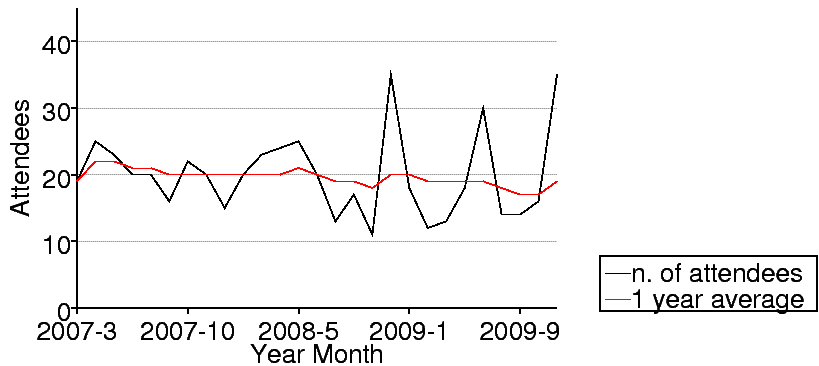
\includegraphics[width=1\hsize]{image200912/kansai.png}
 \end{center}
\caption{関西の参加人数推移}
\label{fig:kansaipeoplechart}
\end{figure}

\begin{table}
\begin{minipage}{0.5\hsize}
 \caption{関西Debian勉強会参加人数(2007年)}\label{tab:count2007kansai}
 \begin{center}
  \begin{tabular}{|l|c|p{10em}|}
 \hline
 & 参加人数 & 内容 \\
 \hline
2007年3月 & 19 & 開催にあたり \\
2007年4月 & 25 & goodbye、youtube、プロジェクトトラッカー\\
2007年6月 & 23 & 社会契約、テーマ、debian/rules、bugreport\\
2007年7月 & 20前後 & OSC-Kansai \\
2007年8月 & 20 & Inkscape、patch、dpatch\\
2007年9月 & 16 & ライブラリ、翻訳、debtorrent\\
2007年10月 & 22& 日本語入力、SPAMフィルタ\\
2007年11月 & 20前後 & KOF \\   
2007年12月 & 15& 忘年会、iPod touch\\   
 \hline
  \end{tabular}
 \end{center}
\end{minipage}
\begin{minipage}{0.5\hsize}
 \caption{関西Debian勉強会参加人数(2008年)}\label{tab:count2008kansai}
 \begin{center}
  \begin{tabular}{|l|c|p{10em}|}
 \hline
 & 参加人数 & 内容 \\
 \hline
2008年2月 & 20 & PC Cluster, GIS, \TeX \\
2008年3月 & 23 & bug report, developer corner, GPG \\
2008年4月 & 24 & coLinux, Debian GNU/kFreeBSD, sid \\
2008年5月 & 25  & ipv6, emacs, ustream.tv\\
2008年6月 & 20  & pbuilder, hotplug, ssl\\
2008年8月 & 13  & coLinux \\
2008年9月 & 17  & debian mentors, ubiquity, DFSG\\
2008年10月 & 11  & cdbs,cdn.debian.or.jp \\
2008年11月 & 35  & KOF \\
2008年12月 & ?  & TeX資料作成ハンズオン\\
 \hline
  \end{tabular}
 \end{center}
\end{minipage}
\begin{minipage}{0.5\hsize}
 \caption{関西Debian勉強会参加人数(2009年)}\label{tab:count2009kansai}
 \begin{center}
  \begin{tabular}{|l|c|p{10em}|}
 \hline
 & 参加人数 & 内容 \\
 \hline
2009年1月 & 18 & DMCK, LT \\
2009年3月 & 12 & Git \\
2009年4月 & 13 & Installing sid, Mancoosi, keysign \\
2009年6月 & 18 & Debian Live, bash\\
2009年7月 & 30? & OSC2009Kansai \\
2009年8月 & 14 & DDTSS, lintian \\
2009年9月 & 14 & reportbug, debian mentors\\
2009年10月 & 16 & gdb, packaging \\
2009年11月 & 35 & KOF2009 \\
2009年12月 & ?? & GPS program, OpenStreetMap \\
 \hline
  \end{tabular}
 \end{center}
\end{minipage}
\end{table}

\clearpage

\dancersection{今後の予定}{Debian JP}

\subsection{次回の関西Debian勉強会}
次回、2010年2月の関西Debian勉強会は 2月28日に
福島区民センターで行ないます。

\subsection{オープンソースカンファレンス Kansai @ Kobe 2010}

2010年3月13日土曜日にJR神戸駅すぐそばの神戸市産業振興センターにて、
オープンソースカンファレンス Kansai @ Kobe 2010が開催されます。
関西Debian勉強会では、現在参加を検討しています。

% 冊子にするために、4の倍数にする必要がある。
% そのための調整
\dancersection{メモ}{}
\mbox{}\newpage

\printindex
 \cleartooddpage

 \begin{minipage}[b]{0.2\hsize}
  \rotatebox{90}{\fontsize{80}{80} {\gt 関西デビアン勉強会} }
 \end{minipage}
 \begin{minipage}[b]{0.8\hsize}

 \vspace*{15cm}
 \rule{\hsize}{1mm}
 \vspace{2mm}
 
\includegraphics[width=2cm]{image200502/openlogo-nd.eps}
 \noindent \Large \bf Debian 勉強会資料\\ \\
 \noindent \normalfont \debmtgyear{}年\debmtgmonth{}月\debmtgdate{}日 \hspace{5mm}  初版第1刷発行\\
 \noindent \normalfont 関西 Debian 勉強会 (編集・印刷・発行)\\
 \rule{\hsize}{1mm}
 \end{minipage}

\end{document}
